% Created by tikzDevice version 0.12.3 on 2019-09-26 18:26:36
% !TEX encoding = UTF-8 Unicode
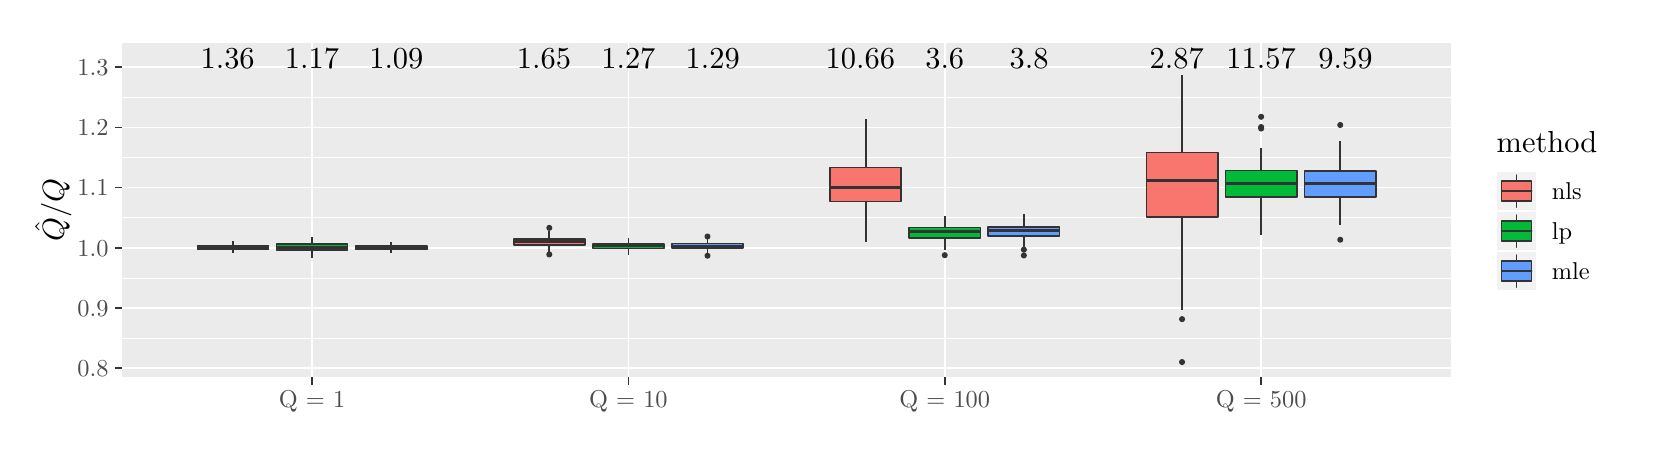
\begin{tikzpicture}[x=1pt,y=1pt]
\definecolor{fillColor}{RGB}{255,255,255}
\path[use as bounding box,fill=fillColor,fill opacity=0.00] (0,0) rectangle (578.16,144.54);
\begin{scope}
\path[clip] (  0.00,  0.00) rectangle (578.16,144.54);
\definecolor{drawColor}{RGB}{255,255,255}
\definecolor{fillColor}{RGB}{255,255,255}

\path[draw=drawColor,line width= 0.6pt,line join=round,line cap=round,fill=fillColor] (  0.00,  0.00) rectangle (578.16,144.54);
\end{scope}
\begin{scope}
\path[clip] ( 34.16, 18.22) rectangle (514.31,139.04);
\definecolor{fillColor}{gray}{0.92}

\path[fill=fillColor] ( 34.16, 18.22) rectangle (514.31,139.04);
\definecolor{drawColor}{RGB}{255,255,255}

\path[draw=drawColor,line width= 0.3pt,line join=round] ( 34.16, 32.36) --
	(514.31, 32.36);

\path[draw=drawColor,line width= 0.3pt,line join=round] ( 34.16, 54.11) --
	(514.31, 54.11);

\path[draw=drawColor,line width= 0.3pt,line join=round] ( 34.16, 75.87) --
	(514.31, 75.87);

\path[draw=drawColor,line width= 0.3pt,line join=round] ( 34.16, 97.63) --
	(514.31, 97.63);

\path[draw=drawColor,line width= 0.3pt,line join=round] ( 34.16,119.39) --
	(514.31,119.39);

\path[draw=drawColor,line width= 0.6pt,line join=round] ( 34.16, 21.48) --
	(514.31, 21.48);

\path[draw=drawColor,line width= 0.6pt,line join=round] ( 34.16, 43.23) --
	(514.31, 43.23);

\path[draw=drawColor,line width= 0.6pt,line join=round] ( 34.16, 64.99) --
	(514.31, 64.99);

\path[draw=drawColor,line width= 0.6pt,line join=round] ( 34.16, 86.75) --
	(514.31, 86.75);

\path[draw=drawColor,line width= 0.6pt,line join=round] ( 34.16,108.51) --
	(514.31,108.51);

\path[draw=drawColor,line width= 0.6pt,line join=round] ( 34.16,130.27) --
	(514.31,130.27);

\path[draw=drawColor,line width= 0.6pt,line join=round] (102.75, 18.22) --
	(102.75,139.04);

\path[draw=drawColor,line width= 0.6pt,line join=round] (217.07, 18.22) --
	(217.07,139.04);

\path[draw=drawColor,line width= 0.6pt,line join=round] (331.39, 18.22) --
	(331.39,139.04);

\path[draw=drawColor,line width= 0.6pt,line join=round] (445.71, 18.22) --
	(445.71,139.04);
\definecolor{drawColor}{gray}{0.20}

\path[draw=drawColor,line width= 0.6pt,line join=round] ( 74.17, 65.87) -- ( 74.17, 67.54);

\path[draw=drawColor,line width= 0.6pt,line join=round] ( 74.17, 64.38) -- ( 74.17, 62.98);
\definecolor{fillColor}{RGB}{248,118,109}

\path[draw=drawColor,line width= 0.6pt,line join=round,line cap=round,fill=fillColor] ( 61.31, 65.87) --
	( 61.31, 64.38) --
	( 87.03, 64.38) --
	( 87.03, 65.87) --
	( 61.31, 65.87) --
	cycle;

\path[draw=drawColor,line width= 1.1pt,line join=round] ( 61.31, 65.05) -- ( 87.03, 65.05);

\path[draw=drawColor,line width= 0.6pt,line join=round] (102.75, 66.26) -- (102.75, 68.74);

\path[draw=drawColor,line width= 0.6pt,line join=round] (102.75, 64.12) -- (102.75, 61.16);
\definecolor{fillColor}{RGB}{0,186,56}

\path[draw=drawColor,line width= 0.6pt,line join=round,line cap=round,fill=fillColor] ( 89.89, 66.26) --
	( 89.89, 64.12) --
	(115.61, 64.12) --
	(115.61, 66.26) --
	( 89.89, 66.26) --
	cycle;

\path[draw=drawColor,line width= 1.1pt,line join=round] ( 89.89, 65.12) -- (115.61, 65.12);

\path[draw=drawColor,line width= 0.6pt,line join=round] (131.33, 65.68) -- (131.33, 66.99);

\path[draw=drawColor,line width= 0.6pt,line join=round] (131.33, 64.43) -- (131.33, 63.21);
\definecolor{fillColor}{RGB}{97,156,255}

\path[draw=drawColor,line width= 0.6pt,line join=round,line cap=round,fill=fillColor] (118.47, 65.68) --
	(118.47, 64.43) --
	(144.19, 64.43) --
	(144.19, 65.68) --
	(118.47, 65.68) --
	cycle;

\path[draw=drawColor,line width= 1.1pt,line join=round] (118.47, 65.18) -- (144.19, 65.18);
\definecolor{fillColor}{gray}{0.20}

\path[draw=drawColor,line width= 0.4pt,line join=round,line cap=round,fill=fillColor] (188.49, 62.59) circle (  0.89);

\path[draw=drawColor,line width= 0.4pt,line join=round,line cap=round,fill=fillColor] (188.49, 72.20) circle (  0.89);

\path[draw=drawColor,line width= 0.6pt,line join=round] (188.49, 68.16) -- (188.49, 71.15);

\path[draw=drawColor,line width= 0.6pt,line join=round] (188.49, 65.99) -- (188.49, 63.11);
\definecolor{fillColor}{RGB}{248,118,109}

\path[draw=drawColor,line width= 0.6pt,line join=round,line cap=round,fill=fillColor] (175.63, 68.16) --
	(175.63, 65.99) --
	(201.35, 65.99) --
	(201.35, 68.16) --
	(175.63, 68.16) --
	cycle;

\path[draw=drawColor,line width= 1.1pt,line join=round] (175.63, 67.23) -- (201.35, 67.23);

\path[draw=drawColor,line width= 0.6pt,line join=round] (217.07, 66.43) -- (217.07, 68.56);

\path[draw=drawColor,line width= 0.6pt,line join=round] (217.07, 64.71) -- (217.07, 62.50);
\definecolor{fillColor}{RGB}{0,186,56}

\path[draw=drawColor,line width= 0.6pt,line join=round,line cap=round,fill=fillColor] (204.21, 66.43) --
	(204.21, 64.71) --
	(229.93, 64.71) --
	(229.93, 66.43) --
	(204.21, 66.43) --
	cycle;

\path[draw=drawColor,line width= 1.1pt,line join=round] (204.21, 65.68) -- (229.93, 65.68);
\definecolor{fillColor}{gray}{0.20}

\path[draw=drawColor,line width= 0.4pt,line join=round,line cap=round,fill=fillColor] (245.65, 69.08) circle (  0.89);

\path[draw=drawColor,line width= 0.4pt,line join=round,line cap=round,fill=fillColor] (245.65, 62.13) circle (  0.89);

\path[draw=drawColor,line width= 0.6pt,line join=round] (245.65, 66.61) -- (245.65, 68.76);

\path[draw=drawColor,line width= 0.6pt,line join=round] (245.65, 64.97) -- (245.65, 63.22);
\definecolor{fillColor}{RGB}{97,156,255}

\path[draw=drawColor,line width= 0.6pt,line join=round,line cap=round,fill=fillColor] (232.79, 66.61) --
	(232.79, 64.97) --
	(258.51, 64.97) --
	(258.51, 66.61) --
	(232.79, 66.61) --
	cycle;

\path[draw=drawColor,line width= 1.1pt,line join=round] (232.79, 65.63) -- (258.51, 65.63);

\path[draw=drawColor,line width= 0.6pt,line join=round] (302.81, 93.98) -- (302.81,111.48);

\path[draw=drawColor,line width= 0.6pt,line join=round] (302.81, 81.73) -- (302.81, 67.13);
\definecolor{fillColor}{RGB}{248,118,109}

\path[draw=drawColor,line width= 0.6pt,line join=round,line cap=round,fill=fillColor] (289.95, 93.98) --
	(289.95, 81.73) --
	(315.67, 81.73) --
	(315.67, 93.98) --
	(289.95, 93.98) --
	cycle;

\path[draw=drawColor,line width= 1.1pt,line join=round] (289.95, 86.92) -- (315.67, 86.92);
\definecolor{fillColor}{gray}{0.20}

\path[draw=drawColor,line width= 0.4pt,line join=round,line cap=round,fill=fillColor] (331.39, 62.33) circle (  0.89);

\path[draw=drawColor,line width= 0.6pt,line join=round] (331.39, 72.36) -- (331.39, 76.37);

\path[draw=drawColor,line width= 0.6pt,line join=round] (331.39, 68.54) -- (331.39, 64.12);
\definecolor{fillColor}{RGB}{0,186,56}

\path[draw=drawColor,line width= 0.6pt,line join=round,line cap=round,fill=fillColor] (318.53, 72.36) --
	(318.53, 68.54) --
	(344.25, 68.54) --
	(344.25, 72.36) --
	(318.53, 72.36) --
	cycle;

\path[draw=drawColor,line width= 1.1pt,line join=round] (318.53, 70.98) -- (344.25, 70.98);
\definecolor{fillColor}{gray}{0.20}

\path[draw=drawColor,line width= 0.4pt,line join=round,line cap=round,fill=fillColor] (359.97, 64.32) circle (  0.89);

\path[draw=drawColor,line width= 0.4pt,line join=round,line cap=round,fill=fillColor] (359.97, 62.23) circle (  0.89);

\path[draw=drawColor,line width= 0.6pt,line join=round] (359.97, 72.50) -- (359.97, 77.26);

\path[draw=drawColor,line width= 0.6pt,line join=round] (359.97, 69.28) -- (359.97, 64.55);
\definecolor{fillColor}{RGB}{97,156,255}

\path[draw=drawColor,line width= 0.6pt,line join=round,line cap=round,fill=fillColor] (347.11, 72.50) --
	(347.11, 69.28) --
	(372.83, 69.28) --
	(372.83, 72.50) --
	(347.11, 72.50) --
	cycle;

\path[draw=drawColor,line width= 1.1pt,line join=round] (347.11, 71.26) -- (372.83, 71.26);
\definecolor{fillColor}{gray}{0.20}

\path[draw=drawColor,line width= 0.4pt,line join=round,line cap=round,fill=fillColor] (417.13, 39.21) circle (  0.89);

\path[draw=drawColor,line width= 0.4pt,line join=round,line cap=round,fill=fillColor] (417.13, 23.71) circle (  0.89);

\path[draw=drawColor,line width= 0.6pt,line join=round] (417.13, 99.47) -- (417.13,127.32);

\path[draw=drawColor,line width= 0.6pt,line join=round] (417.13, 76.06) -- (417.13, 42.40);
\definecolor{fillColor}{RGB}{248,118,109}

\path[draw=drawColor,line width= 0.6pt,line join=round,line cap=round,fill=fillColor] (404.27, 99.47) --
	(404.27, 76.06) --
	(430.00, 76.06) --
	(430.00, 99.47) --
	(404.27, 99.47) --
	cycle;

\path[draw=drawColor,line width= 1.1pt,line join=round] (404.27, 89.42) -- (430.00, 89.42);
\definecolor{fillColor}{gray}{0.20}

\path[draw=drawColor,line width= 0.4pt,line join=round,line cap=round,fill=fillColor] (445.71,108.63) circle (  0.89);

\path[draw=drawColor,line width= 0.4pt,line join=round,line cap=round,fill=fillColor] (445.71,108.09) circle (  0.89);

\path[draw=drawColor,line width= 0.4pt,line join=round,line cap=round,fill=fillColor] (445.71,112.34) circle (  0.89);

\path[draw=drawColor,line width= 0.6pt,line join=round] (445.71, 92.89) -- (445.71,101.08);

\path[draw=drawColor,line width= 0.6pt,line join=round] (445.71, 83.32) -- (445.71, 69.52);
\definecolor{fillColor}{RGB}{0,186,56}

\path[draw=drawColor,line width= 0.6pt,line join=round,line cap=round,fill=fillColor] (432.85, 92.89) --
	(432.85, 83.32) --
	(458.58, 83.32) --
	(458.58, 92.89) --
	(432.85, 92.89) --
	cycle;

\path[draw=drawColor,line width= 1.1pt,line join=round] (432.85, 88.29) -- (458.58, 88.29);
\definecolor{fillColor}{gray}{0.20}

\path[draw=drawColor,line width= 0.4pt,line join=round,line cap=round,fill=fillColor] (474.29, 67.91) circle (  0.89);

\path[draw=drawColor,line width= 0.4pt,line join=round,line cap=round,fill=fillColor] (474.29,109.37) circle (  0.89);

\path[draw=drawColor,line width= 0.6pt,line join=round] (474.29, 92.85) -- (474.29,103.73);

\path[draw=drawColor,line width= 0.6pt,line join=round] (474.29, 83.33) -- (474.29, 73.30);
\definecolor{fillColor}{RGB}{97,156,255}

\path[draw=drawColor,line width= 0.6pt,line join=round,line cap=round,fill=fillColor] (461.43, 92.85) --
	(461.43, 83.33) --
	(487.16, 83.33) --
	(487.16, 92.85) --
	(461.43, 92.85) --
	cycle;

\path[draw=drawColor,line width= 1.1pt,line join=round] (461.43, 88.32) -- (487.16, 88.32);
\definecolor{drawColor}{RGB}{0,0,0}

\node[text=drawColor,anchor=base,inner sep=0pt, outer sep=0pt, scale=  1.10] at (133.23,129.75) {1.09};

\node[text=drawColor,anchor=base,inner sep=0pt, outer sep=0pt, scale=  1.10] at (102.75,129.75) {1.17};

\node[text=drawColor,anchor=base,inner sep=0pt, outer sep=0pt, scale=  1.10] at ( 72.26,129.75) {1.36};

\node[text=drawColor,anchor=base,inner sep=0pt, outer sep=0pt, scale=  1.10] at (247.56,129.75) {1.29};

\node[text=drawColor,anchor=base,inner sep=0pt, outer sep=0pt, scale=  1.10] at (217.07,129.75) {1.27};

\node[text=drawColor,anchor=base,inner sep=0pt, outer sep=0pt, scale=  1.10] at (186.59,129.75) {1.65};

\node[text=drawColor,anchor=base,inner sep=0pt, outer sep=0pt, scale=  1.10] at (361.88,129.75) {3.8};

\node[text=drawColor,anchor=base,inner sep=0pt, outer sep=0pt, scale=  1.10] at (331.39,129.75) {3.6};

\node[text=drawColor,anchor=base,inner sep=0pt, outer sep=0pt, scale=  1.10] at (300.91,129.75) {10.66};

\node[text=drawColor,anchor=base,inner sep=0pt, outer sep=0pt, scale=  1.10] at (476.20,129.75) {9.59};

\node[text=drawColor,anchor=base,inner sep=0pt, outer sep=0pt, scale=  1.10] at (445.71,129.75) {11.57};

\node[text=drawColor,anchor=base,inner sep=0pt, outer sep=0pt, scale=  1.10] at (415.23,129.75) {2.87};
\end{scope}
\begin{scope}
\path[clip] (  0.00,  0.00) rectangle (578.16,144.54);
\definecolor{drawColor}{gray}{0.30}

\node[text=drawColor,anchor=base east,inner sep=0pt, outer sep=0pt, scale=  0.88] at ( 29.21, 18.44) {0.8};

\node[text=drawColor,anchor=base east,inner sep=0pt, outer sep=0pt, scale=  0.88] at ( 29.21, 40.20) {0.9};

\node[text=drawColor,anchor=base east,inner sep=0pt, outer sep=0pt, scale=  0.88] at ( 29.21, 61.96) {1.0};

\node[text=drawColor,anchor=base east,inner sep=0pt, outer sep=0pt, scale=  0.88] at ( 29.21, 83.72) {1.1};

\node[text=drawColor,anchor=base east,inner sep=0pt, outer sep=0pt, scale=  0.88] at ( 29.21,105.48) {1.2};

\node[text=drawColor,anchor=base east,inner sep=0pt, outer sep=0pt, scale=  0.88] at ( 29.21,127.24) {1.3};
\end{scope}
\begin{scope}
\path[clip] (  0.00,  0.00) rectangle (578.16,144.54);
\definecolor{drawColor}{gray}{0.20}

\path[draw=drawColor,line width= 0.6pt,line join=round] ( 31.41, 21.48) --
	( 34.16, 21.48);

\path[draw=drawColor,line width= 0.6pt,line join=round] ( 31.41, 43.23) --
	( 34.16, 43.23);

\path[draw=drawColor,line width= 0.6pt,line join=round] ( 31.41, 64.99) --
	( 34.16, 64.99);

\path[draw=drawColor,line width= 0.6pt,line join=round] ( 31.41, 86.75) --
	( 34.16, 86.75);

\path[draw=drawColor,line width= 0.6pt,line join=round] ( 31.41,108.51) --
	( 34.16,108.51);

\path[draw=drawColor,line width= 0.6pt,line join=round] ( 31.41,130.27) --
	( 34.16,130.27);
\end{scope}
\begin{scope}
\path[clip] (  0.00,  0.00) rectangle (578.16,144.54);
\definecolor{drawColor}{gray}{0.20}

\path[draw=drawColor,line width= 0.6pt,line join=round] (102.75, 15.47) --
	(102.75, 18.22);

\path[draw=drawColor,line width= 0.6pt,line join=round] (217.07, 15.47) --
	(217.07, 18.22);

\path[draw=drawColor,line width= 0.6pt,line join=round] (331.39, 15.47) --
	(331.39, 18.22);

\path[draw=drawColor,line width= 0.6pt,line join=round] (445.71, 15.47) --
	(445.71, 18.22);
\end{scope}
\begin{scope}
\path[clip] (  0.00,  0.00) rectangle (578.16,144.54);
\definecolor{drawColor}{gray}{0.30}

\node[text=drawColor,anchor=base,inner sep=0pt, outer sep=0pt, scale=  0.88] at (102.75,  7.21) {Q = 1};

\node[text=drawColor,anchor=base,inner sep=0pt, outer sep=0pt, scale=  0.88] at (217.07,  7.21) {Q = 10};

\node[text=drawColor,anchor=base,inner sep=0pt, outer sep=0pt, scale=  0.88] at (331.39,  7.21) {Q = 100};

\node[text=drawColor,anchor=base,inner sep=0pt, outer sep=0pt, scale=  0.88] at (445.71,  7.21) {Q = 500};
\end{scope}
\begin{scope}
\path[clip] (  0.00,  0.00) rectangle (578.16,144.54);
\definecolor{drawColor}{RGB}{0,0,0}

\node[text=drawColor,rotate= 90.00,anchor=base,inner sep=0pt, outer sep=0pt, scale=  1.10] at ( 13.08, 78.63) {$\hat{Q}/Q$};
\end{scope}
\begin{scope}
\path[clip] (  0.00,  0.00) rectangle (578.16,144.54);
\definecolor{fillColor}{RGB}{255,255,255}

\path[fill=fillColor] (525.31, 43.84) rectangle (572.66,113.42);
\end{scope}
\begin{scope}
\path[clip] (  0.00,  0.00) rectangle (578.16,144.54);
\definecolor{drawColor}{RGB}{0,0,0}

\node[text=drawColor,anchor=base west,inner sep=0pt, outer sep=0pt, scale=  1.10] at (530.81, 99.27) {method};
\end{scope}
\begin{scope}
\path[clip] (  0.00,  0.00) rectangle (578.16,144.54);
\definecolor{drawColor}{RGB}{255,255,255}
\definecolor{fillColor}{gray}{0.95}

\path[draw=drawColor,line width= 0.6pt,line join=round,line cap=round,fill=fillColor] (530.81, 78.25) rectangle (545.26, 92.70);
\end{scope}
\begin{scope}
\path[clip] (  0.00,  0.00) rectangle (578.16,144.54);
\definecolor{drawColor}{gray}{0.20}

\path[draw=drawColor,line width= 0.6pt,line join=round,line cap=round] (538.03, 79.70) --
	(538.03, 81.86);

\path[draw=drawColor,line width= 0.6pt,line join=round,line cap=round] (538.03, 89.09) --
	(538.03, 91.26);
\definecolor{fillColor}{RGB}{248,118,109}

\path[draw=drawColor,line width= 0.6pt,line join=round,line cap=round,fill=fillColor] (532.61, 81.86) rectangle (543.45, 89.09);

\path[draw=drawColor,line width= 0.6pt,line join=round,line cap=round] (532.61, 85.48) --
	(543.45, 85.48);
\end{scope}
\begin{scope}
\path[clip] (  0.00,  0.00) rectangle (578.16,144.54);
\definecolor{drawColor}{RGB}{255,255,255}
\definecolor{fillColor}{gray}{0.95}

\path[draw=drawColor,line width= 0.6pt,line join=round,line cap=round,fill=fillColor] (530.81, 63.80) rectangle (545.26, 78.25);
\end{scope}
\begin{scope}
\path[clip] (  0.00,  0.00) rectangle (578.16,144.54);
\definecolor{drawColor}{gray}{0.20}

\path[draw=drawColor,line width= 0.6pt,line join=round,line cap=round] (538.03, 65.24) --
	(538.03, 67.41);

\path[draw=drawColor,line width= 0.6pt,line join=round,line cap=round] (538.03, 74.64) --
	(538.03, 76.81);
\definecolor{fillColor}{RGB}{0,186,56}

\path[draw=drawColor,line width= 0.6pt,line join=round,line cap=round,fill=fillColor] (532.61, 67.41) rectangle (543.45, 74.64);

\path[draw=drawColor,line width= 0.6pt,line join=round,line cap=round] (532.61, 71.02) --
	(543.45, 71.02);
\end{scope}
\begin{scope}
\path[clip] (  0.00,  0.00) rectangle (578.16,144.54);
\definecolor{drawColor}{RGB}{255,255,255}
\definecolor{fillColor}{gray}{0.95}

\path[draw=drawColor,line width= 0.6pt,line join=round,line cap=round,fill=fillColor] (530.81, 49.34) rectangle (545.26, 63.80);
\end{scope}
\begin{scope}
\path[clip] (  0.00,  0.00) rectangle (578.16,144.54);
\definecolor{drawColor}{gray}{0.20}

\path[draw=drawColor,line width= 0.6pt,line join=round,line cap=round] (538.03, 50.79) --
	(538.03, 52.96);

\path[draw=drawColor,line width= 0.6pt,line join=round,line cap=round] (538.03, 60.18) --
	(538.03, 62.35);
\definecolor{fillColor}{RGB}{97,156,255}

\path[draw=drawColor,line width= 0.6pt,line join=round,line cap=round,fill=fillColor] (532.61, 52.96) rectangle (543.45, 60.18);

\path[draw=drawColor,line width= 0.6pt,line join=round,line cap=round] (532.61, 56.57) --
	(543.45, 56.57);
\end{scope}
\begin{scope}
\path[clip] (  0.00,  0.00) rectangle (578.16,144.54);
\definecolor{drawColor}{RGB}{0,0,0}

\node[text=drawColor,anchor=base west,inner sep=0pt, outer sep=0pt, scale=  0.88] at (550.76, 82.45) {nls};
\end{scope}
\begin{scope}
\path[clip] (  0.00,  0.00) rectangle (578.16,144.54);
\definecolor{drawColor}{RGB}{0,0,0}

\node[text=drawColor,anchor=base west,inner sep=0pt, outer sep=0pt, scale=  0.88] at (550.76, 67.99) {lp};
\end{scope}
\begin{scope}
\path[clip] (  0.00,  0.00) rectangle (578.16,144.54);
\definecolor{drawColor}{RGB}{0,0,0}

\node[text=drawColor,anchor=base west,inner sep=0pt, outer sep=0pt, scale=  0.88] at (550.76, 53.54) {mle};
\end{scope}
\end{tikzpicture}
